\section{Regulære udtryk og automater}

\subsection{Årsager til at automaten er ikke–deterministisk}

Automaten er ikke deterministisk fordi:

\begin{enumerate}
    \item Der går 2 \texttt{a}-kanter ud fra knude 1
    \item Der går 2 \texttt{b}-kanter ud fra knude 2
    \item Der går en $\epsilon$-kant fra knude 3 til knude 4
\end{enumerate}

\subsection{Eksempler på genkendelige strenge}

Disse strenge bliver genkendt af automaten:

\begin{enumerate}
    \item \texttt{ab}
    \item \texttt{abb}
    \item \texttt{aaaaab}
\end{enumerate}

Der findes uendeligt mange flere.

\subsection{Beskrivelse af sproget}

Sproget, som automaten genkender, starter altid med et \texttt{a}. Derefter kommer der muligvis et \texttt{b}. Derefter kommer der mellem 0 til uendeligt \texttt{a}'er. Til sidst kommer der altid et \texttt{b}.

\subsection{Konvertering til DFA}

Forneden ses en systematisk konstruktion af DFA'en jf. Introduction to Compiler Design samt David Christiansens vejledning. Et $\times$ indikerer, at der ikke findes en overgang. En tilstand med \underline{streg under} indikerer en accepterende tilstand.

\begin{table}[H]
    \centering
    \begin{tabular}{llll}
        \toprule
         DFA-tilstand & Ved \texttt{a} & Ved \texttt{b} & NFA-tilstande \\
         \midrule
         $s_1$ & $s_2$ & $\times$ & $\{ 1 \}$ \\
         $s_2$ & $s_3$ & $s_4$ & $\{ 2, 3, 4 \}$ \\
         $s_3$ & $s_3$ & $s_5$ & $\{ 4 \}$ \\
         $\underline{s_4}$ & $s_3$ & $s_5$ & $\{ 3, 4, \underline{5} \}$ \\
         $\underline{s_5}$ & $\times$ & $\times$ & $\{ \underline{5} \}$ \\
         \bottomrule
    \end{tabular}
\end{table}

Den konstruerede DFA er tegnet således:

\begin{figure}[H]
    \centering
    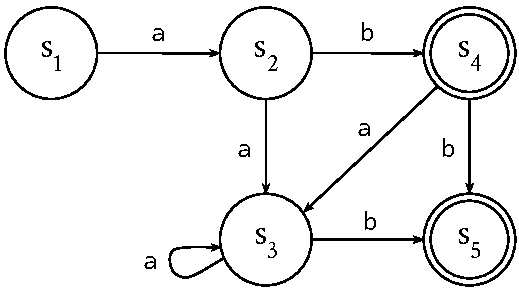
\includegraphics[scale=0.8]{2019-dec/figs/dfa.pdf}
\end{figure}
